\section{ASE Modellen} 
\noindent Den udviklingsmodel, som primært er brugt i projektet, er ASE modellen som ses på figur \ref{fig:ASE}. ASE modellen er en mellemvægtig semi-iterativ udviklingsmodel, som er drevet ud fra en kravspecifikation, der bygger på user stories. ASE modellen tager udgangspunkt i vandfaldsmodellen til at opbygge dit projekt gennem faserne: Projektformulering - Kravspecifikation - Systemarkitektur -  Implementering -  Test/fejlfinding -  Integration og vedligeholdelse.

\begin{figure} [!ht]
	\begin{center}
		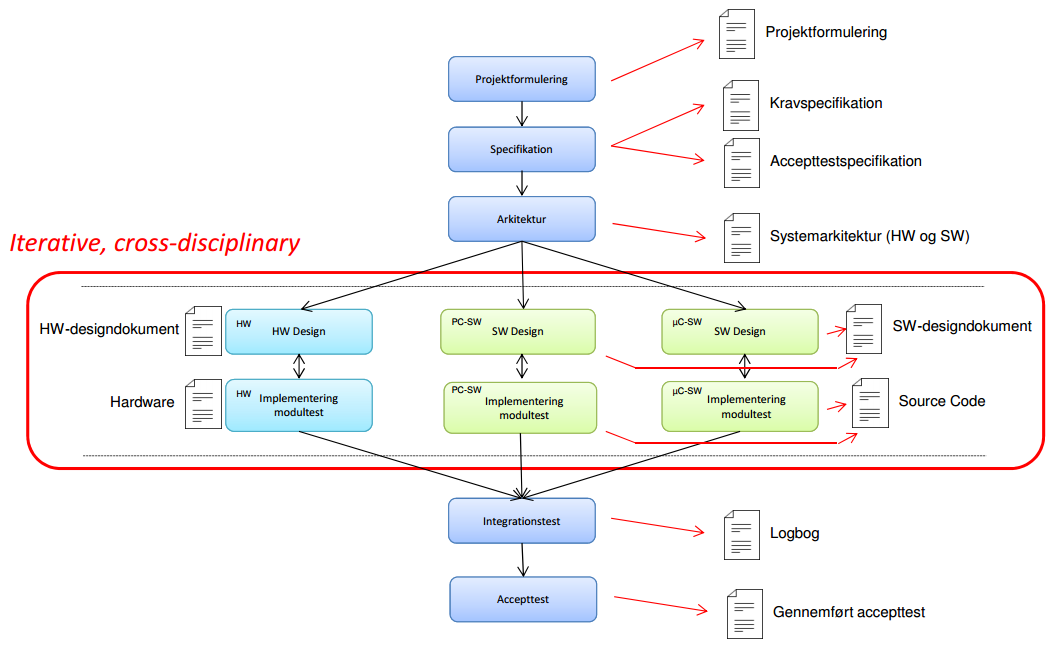
\includegraphics[height=10cm, width=12cm]{Projektbeskrivelse/subpages/ASEModellen.png}
	\end{center}
	\caption{ASE modellen \cite{ASE}}
	\label{fig:ASE}
\end{figure}

\noindent Første punkt i ASE modellen, er at få skrevet en projektformulering og herefter en kravspecifikation, som består af en række user stories. User stories er et værktøj, der beskriver, hvordan der interageres med systemet. Efterfølgende opbygges en kravspecifikation ud fra user stories, og herved opnås et godt overblik over, hvilke krav der er til systemet. Accepttesten specificeres derefter ud fra kravspecifikationen, så alle dele i det samlede system bliver testet.
Når kravspecifikationen er udarbejdet påbegyndes udarbejdningen af systemarkitekturen. I systemarkitekturen skematiserer systemets moduler og grænseflader til de andre moduler i systemet. Når den overordnede arkitektur er på plads, brydes systemet op efter funktionalitet, og designes i forhold til hard- og software. \\

\section{UML, Design og Test}
Der er brugt forskellige teknikker og værktøjer til at gennemføre projekt. Disse beskrives i afsnittene her under.
\subsection{UML}
Software designet er der blevet taget udgangspunkt i en domænemodel og UML klasse diagrammer til at vise og specificere, hvordan grænsefladerne mellem modulerne er på softwaresiden.
Ved hjælp af domænenmodellen udvikles softwareklasser og hvordan de interagere med hinanden.
Domænemodellen giver et godt overblik over, hvordan de forskellige klasser skal arbejde i systemet. Derudover viser den grænseflader, som står for at fortælle, hvordan de forskellige klasser skal kommunikere med hinanden.

\subsection{Design}
Software design er et værktøj der bruges blandt udviklere til at skabe software på den bedst mulige måde. Der er mange overvejelser der skal gøres ved valget af design. Dette bliver ofte diskuteret i grupper, for at alle er enige om hvordan udviklingen skal gribes an og der bruges samme design fra start.

\subsection{Test}
Softwaretest bruges til at sikre en god kvalitet i koden der bliver udviklet. Ved at skrive tests til koden, opdages fejl i kodens opførsel. Hvilket før det muligt at finde fejl før udgivelse.
\newline

\section{Projektstyring}
Styringen af dette projekt, er sket gennem ugentlige møder i gruppen, eventuelt med vejleder.
Projektet strækker sig over et helt semester.  Da det samtidig er sideløbende med undervisningen, danner ASE modellen et godt grundlag for styring af dette projekt. 
Der er gennem projektet blevet arbejdet iterativt med udvikling af både dokumentation, rapport og prototypen, da der løbende har været revurderinger af tidligere arbejde og efterfølgende optimeringer eller ændringer. 
Rollerne i gruppen har gennem projektet skiftet hænder, så alle har prøvet at have alle roller og haft en føling med hele projektet.

Da den overordnede funktionalitet af systemet skulle bestemmes, sad hele gruppen og arbejdede i fællesskab, for at nå frem til et produkt, alle var tilfredse med.
Alle har derfor været inde over kravene til systemet, og den grundlæggende opbygning af arkitekturen.
Efter alt det overordnede var blevet fastlagt, og alle var tilfredse med systemet, deltes gruppen op og arbejdede med design og implementering.
Der har været to faste dage, hvor der blev arbejdet med projektet. Her blev ugens problemstillinger lagt op, og der blev holdt et lille møde med inputs, og opdateringer på, hvor langt folk var, og hvordan disse problemstillinger kunne løses. \\
Der er blevet brugt Git til at styre versionshistorikken på alle dokumenter og software. 

Da gruppen altid sad samlet, var der god kommunikation om hvor langt de forskellige grupper var med deres pågældende område,  derfor vidste en gruppe som stod uden arbejde hurtigt hvor de skulle tage fat.
Dette gav en god iterativ arbejdsproces da ændringer hos en gruppe, hurtigt blev kommunikeret videre til resten af gruppen. 
Hvis kravene til systemet viste sig uhensigtsmæssige, blev disse løbende ændret. \\

